\section{Signale und Systeme}
	\begin{tabular}{|l|l|}
    	\hline
    	\textbf{Linearität} & \textbf{Zeitinvarianz}\\
    	\hline
    	$S(x1+x2)=S(x1)+S(x2)$ & $S(x(t-t_0)=S(x)\cdot x(t-t_0)$ \\
    	$S(c\cdot x)=c\cdot S(x)$ & \\
		\hline    
    \end{tabular}
  	
	\subsection{Lineare Systeme}
		\textbf{Basissignale}
		\begin{list}{$\bullet$}{\setlength{\itemsep}{0cm} \setlength{\parsep}{0cm} \setlength{\topsep}{0cm}} 
          \item Lineare Systeme sind durch die Antworten auf die
          Basissignale bestimmt.
          \item Basissignale müssen linear unabhängig voneinander sein, d.h. ein
		Basissignal darf nicht durch \textbf{Linearkombination} anderer Basissignale
		darstellbar sein          
		  \item Alle möglichen Eingangs-Funktionen müssen durch eine Linearkombination der
		Basissignale dargestellt werden können. $\Rightarrow$ \textbf{Periode des Eingangssignals =	Anzahl Basissignale}
        \end{list}
        \vspace{.2cm}
		\textbf{Berechnung der Systemantwort aufgrund der Basissignale und der
		Anregung}\\
		1. Eingangssignal $x$ als Linearkombination der Basisvektoren darstellen
		$\Rightarrow$ lineares Gleichungssystem\\
		$\Rightarrow x=r\cdot a + s\cdot b + t\cdot c\qquad$ ($x=$
		Eingangssignal; $a,b,c=$ Basisvektoren; $r,s,t=$
		Linearkombinationsparameter)\\ 
		2. Systemantwort $y=r\cdot S(a) + s\cdot S(b) + t\cdot S(c); \qquad (S(a)=$
		Systemantwort der Basis $a$)
	
	\subsection{Lineare zeitinvariante Systeme (LTI-Systeme)}
		LTI-Systeme sind durch ihre Impulsantwort $h$ vollständig bestimmt\\ \\
		\textbf{Berechnung der Systemantwort von diskreten LTI-Systemen}\\
		$\; y=x*h \qquad$ ($y=$ Systemantwort; $x=$ Eingangssignal; $h=$
		Impulsantwort)\\
		
		\textbf{Berechnung der Systemantwort von kontinuierlichen LTI-Systemen}\\
		\begin{tabular}{ll}
			\parbox{8cm}{
			$$s_2(t) = h(t) * s_1(t) \laplace S_2(s) = H(s) S_1(s)$$
			$$h(t) \laplace H(s)$$}
			& \parbox{8cm}{
			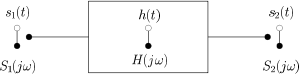
\includegraphics[width=5cm]{./bilder/utf-theorie.png}}\\
		\end{tabular}	
		
	\subsection{Faltung}
		\begin{tabular}{ll}
	        $\boxed{y=x*h=h*x}$&$h=$Impulsantwort des Systems\\ & \\
	   		\textbf{diskret}& \textbf{kontinuierlich}\\
	   		$\boxed{y(i)=\sum\limits_{k=-\infty}^{\infty}x(k)\cdot
	   		h(i-k)=\sum\limits_{k=-\infty}^{\infty}x(i-k)\cdot h(k)}$&
	   		$\boxed{y(t)=\int\limits_{-\infty}^{\infty}x(\tau)\cdot
	   		h(t-\tau)\cdot d\tau=\int\limits_{-\infty}^{\infty}x(t-\tau)\cdot
	   		h(\tau)\cdot d\tau}$\\ & \\
	   		grafische Interpretation: & grafische Interpretation:\\
	   		\parbox{8cm}{1. einfacheres Signal an der Y-Achse spiegeln\\
	   					2. Verschiebung um  $i$ nach rechts\\
	   					3. Skalarprodukt der beiden Signale bilden}&
			\parbox{8cm}{1. einfacheres Signal an der Y-Achse spiegeln\\
			 			2. Verschiebung um $t$ nach rechts\\
			 			3. Multiplikation und Integration der beiden Signale}		
        \end{tabular}
	